\chapter{Revisão Bibliográfica}\label{cap:revbib}

% \MexerDepois{Escrever algo aqui}

Este capítulo apresenta a fundamentação teórica utilizada ao longo do trabalho, bem como um breve levantamento de trabalhos relacionados, que mostram a relevância do assunto abordado.

\section{Fundamentação Teórica}

% \MexerDepois{Completar isso depois}

A construção deste trabalho fundamentou-se em princípios teóricos, envolvendo princípios de codificações de cores, apresentadas na \autoref{ssec:cores}, princípios de visão computacional, apresentados na \autoref{ssec:visao}, e uma ampla utilização do banco digital de bulas eletrônicas da \ac{Anvisa}, apresentado na \autoref{ssec:db}.

\subsection{Codificação de cores}\label{ssec:cores}

Os olhos humanos possuem receptores para cores, chamados cones, divididos em três grupos de sensibilidade, para vermelho, verde e azul \cite{gonzalez2008digital}.
Em alguns casos excepcionais, é possível encontrar mais ou menos grupos de cones em uma pessoa, conforme características genéticas dela \cite{connell2019ColorBlindness, timjewell2023Tetrachromacy}.
Baseada na característica dos olhos, em 1931, a \ac{CIE} padronizou cores vermelho, verde e azul como primárias aditivas, esse sistema é chamado \ac{RGB}.
Apesar dessa denominação, essas cores fixas não são capazes de gerar todo o espectro de cores que os olhos podem perceber \cite{gonzalez2008digital}.

A junção das cores primárias forma as chamadas cores secundárias, então ciano da junção de verde com azul, magenta da junção de azul com vermelho, e amarelo da junção de vermelho com verde.
Juntar as três cores primárias, ou uma primária com sua complementar, forma a cor branca.
Na ausência de luz, é definida a cor preta.
Essas propriedades são aplicáveis para as cores aditivas \cite{gonzalez2008digital}.
A \autoref{fig:cores:rgb} apresenta a representação da codificação RGB.

Existem também as cores primárias para pigmentos, que, diferente das aditivas, operam pela lógica de absorver (subtrair) componentes das cores primárias aditivas, refletindo as demais cores do espectro.
As cores utilizadas são ciano, magenta e amarelo, atualmente é comum também utilizar o pigmento preto, para auxiliar no contraste, esse sistema é chamado \ac{CMYK}.
Complementarmente, as cores secundárias são formadas pela junção destes pigmentos, então vermelho da junção de magenta com amarelo, verde com a junção de ciano com amarelo, e azul da junção de ciano com magenta.
Na ausência de pigmentos, é definida a cor branca.
Essas propriedades são aplicáveis para as cores subtrativas \cite{gonzalez2008digital}.
A \autoref{fig:cores:cmyk} apresenta a representação da codificação \ac{CMYK}.

\begin{figure}[htbp]
    \centering
    \caption{Sistemas de codificação de cores aditivo (\subref{fig:cores:rgb}) e subtrativo (\subref{fig:cores:cmyk}).}
    \label{fig:cores}
    \hfill
    \begin{subfigure}[c]{0.45\textwidth}
        \centering
        % \begin{tikzpicture}[radius=1.5cm]

    \coordinate (O) at (0,0);
    
    % \draw [help lines, dashed] (-3,-3) grid (3,3); % desenha grid
    % \draw [red] (O) node[draw,cross out] {}; % marca pont(0,0) 
    
    % \path[fill=Black] (-2.5,-2.5) rectangle (2.5,2.5);
    \path[draw=rgb_K, fill=rgb_K] circle[radius=3cm];
    % \clip (-6.8,-4) rectangle (6.8,4);

  % \draw (0,0)  arc[start angle=180, end angle=90]
  %     (2,.5) arc[start angle=90,  delta angle=-90];
  % \draw (4,0) -- +(30:1cm)
  %             arc [start angle=30,  delta angle=30] -- cycle;
  % \draw (8,0) arc [start angle=0,   end angle=270,
  %                  x radius=1cm, y radius=5mm] -- cycle;

    % \path[draw, fill=green] (150:1) arc[start angle=180, end angle=90];
    
    \coordinate (cG) at (90 :0.866);
    \coordinate (cR) at (210:0.866);
    \coordinate (cB) at (330:0.866);

    % \path[draw=green, thick] (cG) circle;
    % \path[draw=red,   thick] (cR) circle;
    % \path[draw=blue,  thick] (cB) circle;

    \path[draw=rgb_R, fill=rgb_R]
        (cR) arc (240:180:1.5)
        arc (120:300:1.5)
        arc (240:180:1.5)
    ;

    \path[draw=rgb_G, fill=rgb_G]
        (cG) arc (120:60:1.5)
        arc (0:180:1.5)
        arc (120:60:1.5)
    ;

    \path[draw=rgb_B, fill=rgb_B]
        (cB) arc (0:-60:1.5)
        arc (-120:60:1.5)
        arc (0:-60:1.5)
    ;

    \path[draw=rgb_C, fill=rgb_C]
        (cG) arc (120:60:1.5)
        arc (0:-60:1.5)
        arc (0:60:1.5)
    ;
    
    \path[draw=rgb_M, fill=rgb_M]
        (cB) arc (0:-60:1.5)
        arc (240:180:1.5)
        arc (240:300:1.5)
    ;
    
    \path[draw=rgb_Y, fill=rgb_Y]
        (cR) arc (240:180:1.5)
        arc (120:60:1.5)
        arc (120:180:1.5)
    ;

    \path[draw=rgb_W, fill=rgb_W]
        (cB) arc (0:60:1.5)
        arc (120:180:1.5)
        arc (240:300:1.5)
    ;
    

    
\end{tikzpicture}
        
\includegraphics{../pictures/RGB.pdf}
        \caption{Sistema aditivo \ac{RGB}.}
        \label{fig:cores:rgb}
    \end{subfigure}
    \hfill
    \begin{subfigure}[c]{0.45\textwidth}
        \centering
        % \begin{tikzpicture}[radius=1.5cm]

    \coordinate (O) at (0,0);
    
    % \draw [help lines, dashed] (-3,-3) grid (3,3); % desenha grid
    % \draw [red] (O) node[draw,cross out] {}; % marca pont(0,0) 
    
    % \path[fill=Black] (-2.5,-2.5) rectangle (2.5,2.5);
    \path[draw=cmyk_K, dashed, fill=cmyk_W] circle[radius=3cm];
    % \clip (-6.8,-4) rectangle (6.8,4);

  % \draw (0,0)  arc[start angle=180, end angle=90]
  %     (2,.5) arc[start angle=90,  delta angle=-90];
  % \draw (4,0) -- +(30:1cm)
  %             arc [start angle=30,  delta angle=30] -- cycle;
  % \draw (8,0) arc [start angle=0,   end angle=270,
  %                  x radius=1cm, y radius=5mm] -- cycle;

    % \path[draw, fill=green] (150:1) arc[start angle=180, end angle=90];
    
    \coordinate (cG) at (90 :0.866);
    \coordinate (cR) at (210:0.866);
    \coordinate (cB) at (330:0.866);

    % \path[draw=green, thick] (cG) circle;
    % \path[draw=red,   thick] (cR) circle;
    % \path[draw=blue,  thick] (cB) circle;

    \path[draw=cmyk_C, fill=cmyk_C]
        (cR) arc (240:180:1.5)
        arc (120:300:1.5)
        arc (240:180:1.5)
    ;

    \path[draw=cmyk_Y, fill=cmyk_Y]
        (cB) arc (0:-60:1.5)
        arc (-120:60:1.5)
        arc (0:-60:1.5)
    ;

    \path[draw=cmyk_M, fill=cmyk_M]
        (cG) arc (120:60:1.5)
        arc (0:180:1.5)
        arc (120:60:1.5)
    ;

    \path[draw=cmyk_R, fill=cmyk_R]
        (cG) arc (120:60:1.5)
        arc (0:-60:1.5)
        arc (0:60:1.5)
    ;
    
    \path[draw=cmyk_G, fill=cmyk_G]
        (cB) arc (0:-60:1.5)
        arc (240:180:1.5)
        arc (240:300:1.5)
    ;
    
    \path[draw=cmyk_B, fill=cmyk_B]
        (cR) arc (240:180:1.5)
        arc (120:60:1.5)
        arc (120:180:1.5)
    ;

    \path[draw=cmyk_K, fill=cmyk_K]
        (cB) arc (0:60:1.5)
        arc (120:180:1.5)
        arc (240:300:1.5)
    ;
    

    
\end{tikzpicture}
        
\includegraphics{../pictures/CMYK.pdf}
        \caption{Sistema subtrativo \ac{CMYK}.}
        \label{fig:cores:cmyk}
    \end{subfigure}
    \hfill
    \caption*{Fonte: Autor.}
\end{figure}

Apesar destes modelos serem amplamente utilizados, eles não representam as cores de uma forma prática para a interpretação humana, já que operam com sobreposições de cores.
Quando uma pessoa vê um objeto, normalmente descreve sua cor pelo tom, saturação e brilho.
O sistema chamado \ac{HSI} é baseado neste princípio, onde a componente de tom indica a cor pura, como azul, roxo ou vermelho, a componente de saturação indica o quão diluída aquela cor está no branco, e a componente de brilho indica quão intensa é a claridade daquela cor.
Este modelo e suas variantes são muito utilizados em ferramentas de processamento de imagens utilizados por humanos, como softwares de edição de foto e vídeo \cite{gonzalez2008digital}.

\subsection{Visão Computacional}\label{ssec:visao}

\citeauthor{haralick1992computer} \cite{haralick1992computer} descrevem visão computacional como a ciência que baseia algoritmos e teorias úteis para extrair automaticamente informações sobre o ambiente analisado através de imagens.
Os métodos possíveis abrangem desde a identificação de objetos genéricos a partir de suas características, bem como a descrição de atributos, como posição e orientação espacial em relação ao ponto de observação.

Uma imagem é a representação espacial bi ou tridimensional de uma cena ou de outra imagem \cite{haralick1992computer}.
No escopo de visão computacional, geralmente se refere a uma imagem capturada, como uma foto, uma figura digital ou um vídeo.
A captura da imagem digital é feita de maneira quantizada, onde o sensor retangular mede a intensidade de luz incidente em sua superfície, geralmente relacionado a um sistema de lentes.

A unidade espacial de uma imagem é o \ac{pixel}, que tem as propriedades de valor e posição, mapeando a informação da imagem.
Seu valor pode ser associado à intensidade de luz naquela região, mas também pode representar informações abstratas, como cores na legenda de uma figura, estas foram imagens denominadas simbólicas.
A \autoref{fig:revisao:simbolica} apresenta uma imagem simbólica.
O valor de intensidade de um \ac{pixel} é chamada do níveis de cinza, geralmente representado por um valor de 8 bits, com valores entre 0 e 255, onde o primeiro representa o preto, tons de cinza para os intermediários e o último o branco

\begin{figure}[htbp]
    \centering
    \caption{Dedicação de tempo com o TCC.}
    \label{fig:revisao:simbolica}
    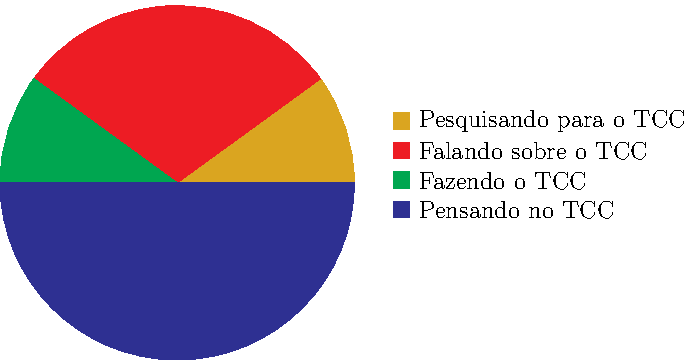
\includegraphics{../pictures/simbolica.pdf}
    % \begin{tikzpicture}
%
\tikzset{
     lines/.style={draw=none},
};%
%
\pie[
        text=legend,
        hide number,
        color={Goldenrod, cmyk_R, cmyk_G, cmyk_B},
        style={lines},
        % rotate=180
    ]{
        10/Pesquisando para o TCC,
        30/Falando sobre o TCC,
        10/Fazendo o TCC,
        50/Pensando no TCC
    };%
    %
\end{tikzpicture}%
    \caption*{Fonte: Autor.}
\end{figure}

Geralmente um \ac{pixel} não é capaz de representar completamente uma entidade numa imagem.
Faz-se necessário um conjunto de \acp{pixel} organizados de forma coerente para tornarem reconhecíveis as características de interesse em um objeto de estudo.
Dentre características de interesse no campo de visão computacional, se destacam formato, cor, tamanho, além de posição e orientação espacial, citadas anteriormente.
A análise dessas características pode levar a identificação do objeto estudado.

Para distinguir objetos do seu entorno e definir sua classificação, é necessário delimitar quais \acp{pixel} fazem ou não parte dele.
Para definir isso, pode ser necessário identificar linhas, curvas e bordas.
Formatos e posições desses atributos podem ser usados como fatores decisivos no momento de identificar o objeto dentre uma lista de possibilidades esperadas.

\subsection{Banco de Dados Sobre Medicamentos}\label{ssec:db}

Em setembro de 2009, a Diretoria Colegiada da \ac{Anvisa} publicou resoluções sobre regulamentação técnica a respeito de requisitos para a elaboração, atualização, publicação e disponibilidade de bulas de medicamentos, garantindo acesso à informação pertinente a pacientes e profissionais de saúde \cite{anvisa2009RDC}.

Em seu portal online, a \ac{Anvisa} disponibiliza acesso ao Bulário Eletrônico, que pode ser consultado sabendo alguma informação sobre o medicamento em questão, dados como o nome do medicamento, o número do registro ou a empresa responsável pela fabricação \cite{anvisa2020bulario}.
A \autoref{fig:bulario_pagina} apresenta a interface da página de buscas.

\begin{figure}[!htbp]
    \centering
    \caption{Página de campos de consulta ao Bulário Eletrônico da \acs{Anvisa}.}
    \label{fig:bulario_pagina}
    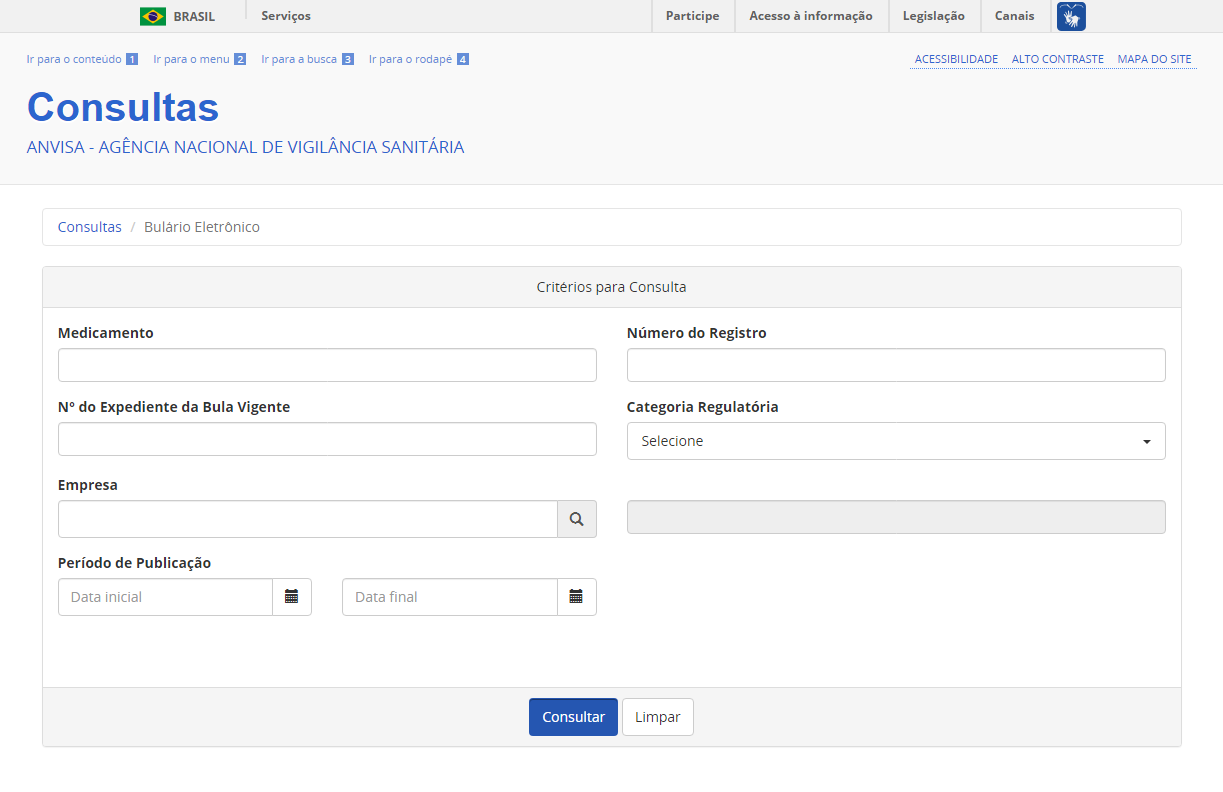
\includegraphics[width=\textwidth]{../pictures/bulario_pagina.png}
    \caption*{Fonte: \href{https://consultas.Anvisa.gov.br/\#/bulario/}{Portal da \ac{Anvisa}}, acesso em 2023-09-06.}
\end{figure}

Para exemplificar a busca, foi escolhido o medicamento TYSABRI\textsuperscript{\tiny\textregistered}.
O nome foi inserido no campo ``Medicamento'' e foi realizada a consulta.
A \autoref{fig:bulario_resultado} apresenta a interface da página com os resultados da busca, neste caso, há apenas um registro no banco de dados da \ac{Anvisa}.

\begin{figure}[!htbp]
    \centering
    \caption[Página de resultados de consulta ao Bulário Eletrônico da \acs{Anvisa}]{Página de resultados de consulta ao Bulário Eletrônico da \acs{Anvisa}, medicamento TYSABRI\textsuperscript{\tiny\textregistered}.}
    \label{fig:bulario_resultado}
    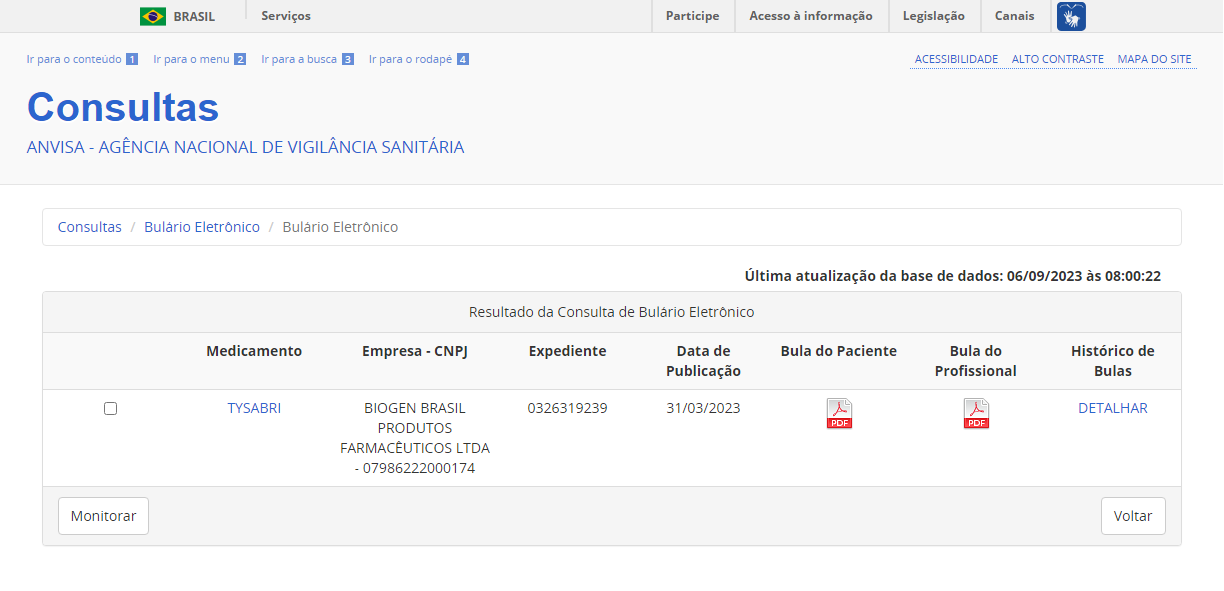
\includegraphics[width=\textwidth]{../pictures/bulario_resultado.png}
    \caption*{Fonte: \href{https://consultas.Anvisa.gov.br/\#/bulario/q/?nomeProduto=TYSABRI}{Portal da \ac{Anvisa}}, acesso em 2023-09-06.}
\end{figure}

Por fim, clicando no nome do medicamento na lista, foi acessada a página de detalhes, apresentada na \autoref{fig:bulario_detalhes}.

\begin{figure}[!htbp]
    \centering
    \caption[Página de detalhes do produto no Bulário Eletrônico da \acs{Anvisa}]{Página de detalhes do produto no Bulário Eletrônico da \acs{Anvisa}, medicamento TYSABRI\textsuperscript{\tiny\textregistered}.}
    \label{fig:bulario_detalhes}
    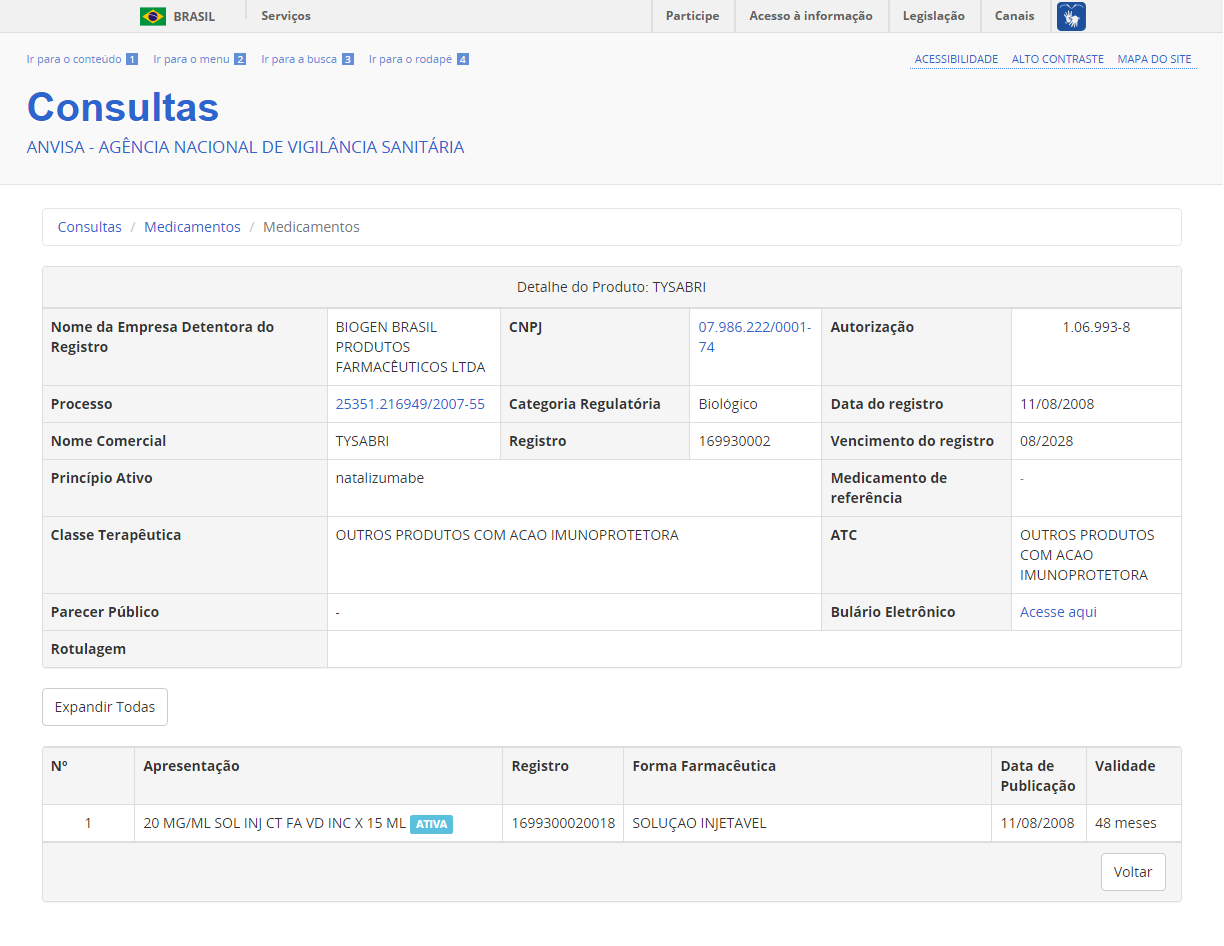
\includegraphics[width=\textwidth]{../pictures/bulario_detalhes.png}
    \caption*{Fonte: \href{https://consultas.Anvisa.gov.br/\#/medicamentos/25351216949200755/}{Portal da \ac{Anvisa}}, acesso em 2023-09-06.}
\end{figure}

Infelizmente o portal da \ac{Anvisa} não disponibiliza uma \ac{API} para acesso ao bulário, o que dificulta o uso deste por programadores e pesquisadores.
Com o objetivo de contornar este problema, \citeauthor{landin2022bulario} \cite{landin2022bulario} criou uma biblioteca em JavaScript que realiza a busca no sistema da \ac{Anvisa} e retorna um objeto JSON com os resultados da busca.

Ainda para ampliar a portabilidade da biblioteca, \citeauthor{landin2022api} também desenvolveu uma \ac{API} para a realização das buscas utilizando requisições web GET \cite{landin2022api}.
O \autoref{cod:sh} apresenta um exemplo de requisição GET para a busca de um medicamento usando o Bulario \ac{API}, e o \autoref{cod:json} apresenta o JSON retornado pela requisição.

\begin{lstfloat}[p]
    \centering
    \lstinputlisting[language=sh, label=cod:sh,
    caption={Exemplo de código de requisição para o medicamento TYSABRI\textsuperscript{\tiny\textregistered} no Bulário \ac{API}.}
    ]{../code/bulario_api.sh}
    \caption*{Fonte: \href{https://bula.vercel.app/docs}{Documentação Bulario \ac{API}}, acesso em 2023-09-06, adaptado.}
\end{lstfloat}

\begin{lstfloat}[p]
    \centering
    \lstinputlisting[language=JavaScript, label=cod:json, caption={Arquivo JSON retornado pela busca ao medicamento TYSABRI\textsuperscript{\tiny\textregistered} no Bulário \ac{API}}]{../code/tysabri.json}
    \caption*{Fonte: \href{https://bula.vercel.app/docs}{Documentação Bulario \ac{API}}, acesso em 2023-09-06, adaptado.}
\end{lstfloat}

% \cite{landin2022api, landin2022bulario, Anvisa2020bulario, Anvisa2009RDC}

\section{Trabalhos Relacionados}

A proposta aqui apresentada já foi explorada anteriormente em outros trabalhos.
Esta seção cita alguns destes, descrevendo propostas, metodologias e dificuldades.

O trabalho apresentado por \citeauthor{steffenon2020katie} \cite{steffenon2020katie} consiste em uma aplicação \textit{mobile}, KATIE, que auxilia pessoas com baixa ou nenhuma visão na realização de tarefas simples.
Esta aplicação tem como objetivo o reconhecer, interpretar e responder perguntas feitas pelo usuário sobre seu ambiente, em alguns casos, com o auxílio da câmera do dispositivo.
A interface com o usuário foi feita baseada em métodos de reconhecimento de fala, bem como conversão da resposta obtida pelo sistema em áudio.
O desenvolvimento teve como enfoque o público alvo, visando ser uma tecnologia assistiva eficiente.
Seus resultados atenderam as expectativas da proposta, conseguindo identificar cédulas de dinheiro e rótulos de medicamentos.

\citeauthor{gadenz2019desenvolvimento} \cite{gadenz2019desenvolvimento} faz uma proposta semelhante a anterior, porém com o enfoque em pessoas acima de 60 anos, tendo em vista que nesta idade, baixas de visão são mais comuns.
A aplicação proposta, além de identificar o medicamento pelo rótulo, também é capaz de fornecer sua bula.
Outra preocupação desse trabalho é relacionada ao risco de efeitos adversos que esses medicamentos podem causar por uso indevido.
Os testes realizados com processamento local, foi obtida uma taxa de acerto de \SI{100}{\percent} para os seis medicamentos cadastrados.

Em sua tese, \citeauthor{benjamim2012identificaccao} \cite{benjamim2012identificaccao} sugere o uso de um sistema para auxiliar a identificação de caixas de medicamentos para pessoas com deficiência visual, com o objetivo de evitar ingestão errônea desses remédios.
A proposta também almeja auxiliar o usuário com detalhes quanto à posologia do medicamento, bem como indicações e contra indicações.
Essa proposta sugere o uso de dispositivos diversos que estariam inseridos do dia a dia dos usuários, desde celulares até televisores.

\citeauthor{rodrigues2022sisamed} \cite{rodrigues2022sisamed} aponta problemas com não adesão ou adesão parcial de pacientes ao uso dos medicamentos, e propõe um sistema capaz de reconhecer automaticamente estes remédios, além de lembrar o paciente nos horários que estes dever ser tomados.
Esta proposta se baseia no uso de um microcomputador, acoplado a uma \textit{webcam} apontada para a superfície onde os medicamentos seriam reservados.
O sistema alertará o paciente no horário correto para que o remédio seja tomado, interrompendo o alerta somente quando detectar que houve interação com o medicamento sobre a mesa.


